\documentclass{article}
\usepackage{graphicx}
\usepackage{amssymb}
\begin{document}
	In a scenario like \texttt{npole} (Fig.~\ref{fig:npole}) the boresight of 
	the spacecraft must form a right angle with the ecliptic.
	The typical way that this scenario is described -- `just rotate the 
	spacecraft $36^\circ$ about spacecraft $+Y$' (cf. 
	Fig.~\ref{fig:spacecraft_angles}) -- is probably wrong.
	
	This is because such a rotation would put Camera 4 only $45^\circ$ in 
	ecliptic latitude away from pointing directly at the Sun.
	Following the lens hood model (Fig.~\ref{fig:lens_hood_suppression}) this 
	means $\sim 10^{-7}$ suppression, or around 18 magnitudes.
  The Sun has $V=-26$, which means with suppresion it's a source with 
  $V=-8$ spread `uniformly' (not actually uniform, but OK for OOM 
  calculations).
  Winn 2013's tabulation of the photon fluxes indicates an $I=0$ G2V star 
  produces $1.6\times 10^6\,\mathrm{ph/s/cm^2}$. 
  Saying V=I, being 8 mags brighter than $I=0$ means $\sim\!1600\times$ as 
  much 
  flux, or 
  $2.5 \times 10^9\,\mathrm{ph/s/cm^2}$.
	Since each lens has an effective observing area of $69\,\mathrm{cm^2}$, this 
	gives $1.7\times 10^{11}\,\mathrm{ph/s}$ across an entire lens.
	The requirements are quoted in ct/s/px, so divide by 
	$4096^2\,\mathrm{px^2}$, and get $10^4\,\mathrm{ph/s/px}$. 100\% QE brings 
	$10^4\,\mathrm{ct/s/px}$.
	This is $\sim\!30\times$ the `treshold' we set when noting `risky fields' 
	for dropping 
	in Bouma et al Sec1.6, and means (multiply by 2 to get the mean ct/px per 2 
	sec image, then take a sqrt to estimate the variance) an additional $\sim\! 
	140 $
	ct/px RMS per 2 sec image.
	This is Bad. It means $\sim 50\%$ of stars that could be observed at 
	sub-mmag precision over 1hr no longer can (cf precision plot and text of 
	Bouma et al 2016). It means $10\times$ worse precision for M dwarfs 
	($I\gtrsim 13$).
	
	We can get around this -- somewhat -- by doing a different rotation.
	Start from the configuration shown in Fig.~\ref{fig:spacecraft_angles}, and 
	rotate by $36^\circ$ about 
	spacecraft $+Y$. Then rotate by $90^\circ$ about spacecraft $+Z$ (same as 
	ecliptic pole direction). All cameras are then $90^\circ$ from the 
	antisolar direction.
	The lens hood model says we now get a suppression of $10^{-9}$, or 23 
	magnitudes, so the sun is $V=-3$, uniformly spread.
	Repeating the calculation, this gives $10^2\,\mathrm{ct/s/px}$, 
	or an additional $\sim\!14 $ ct/px RMS per 2 sec image.
	This isn't great, and is a slight hit on M dwarf precision, but it's way 
	preferable to the scenario described above.
	However, an obvious problem with this arrangement is that it must block 
	at least one solar panel, unless I am missing something.
	
	When we chatted about this, you mentioned it wouldn't be a problem. 
	{\bf Am I missing something?}
	
	
	
	\begin{figure}[!h]
		\centering
		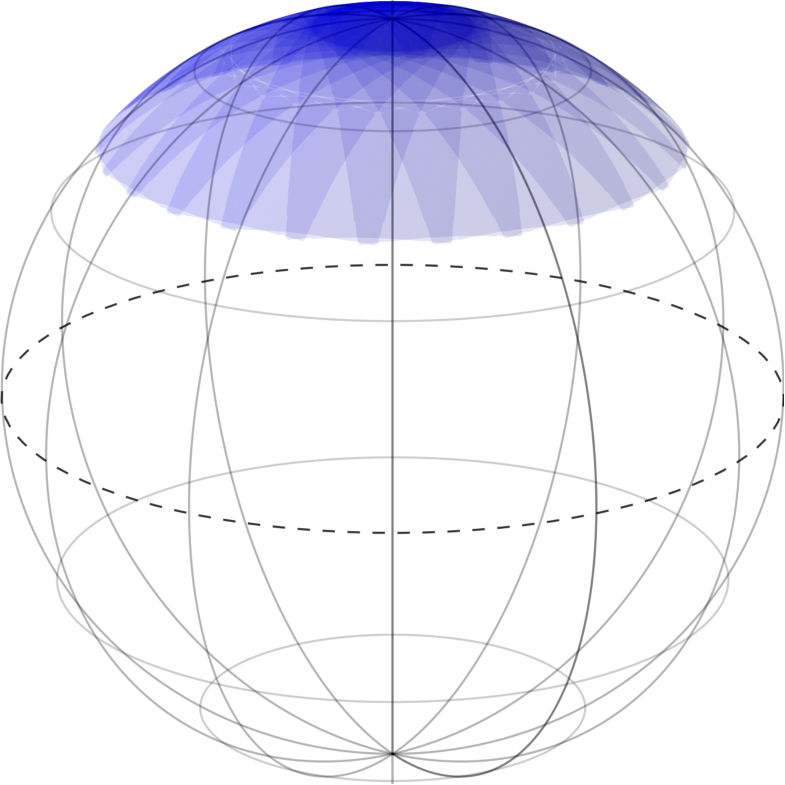
\includegraphics[width=0.3\textwidth]{../figures/npole.pdf}
		\caption{\texttt{npole} scenario}
		\label{fig:npole}
	\end{figure}
	
	\begin{figure}[!b]
		\centering
		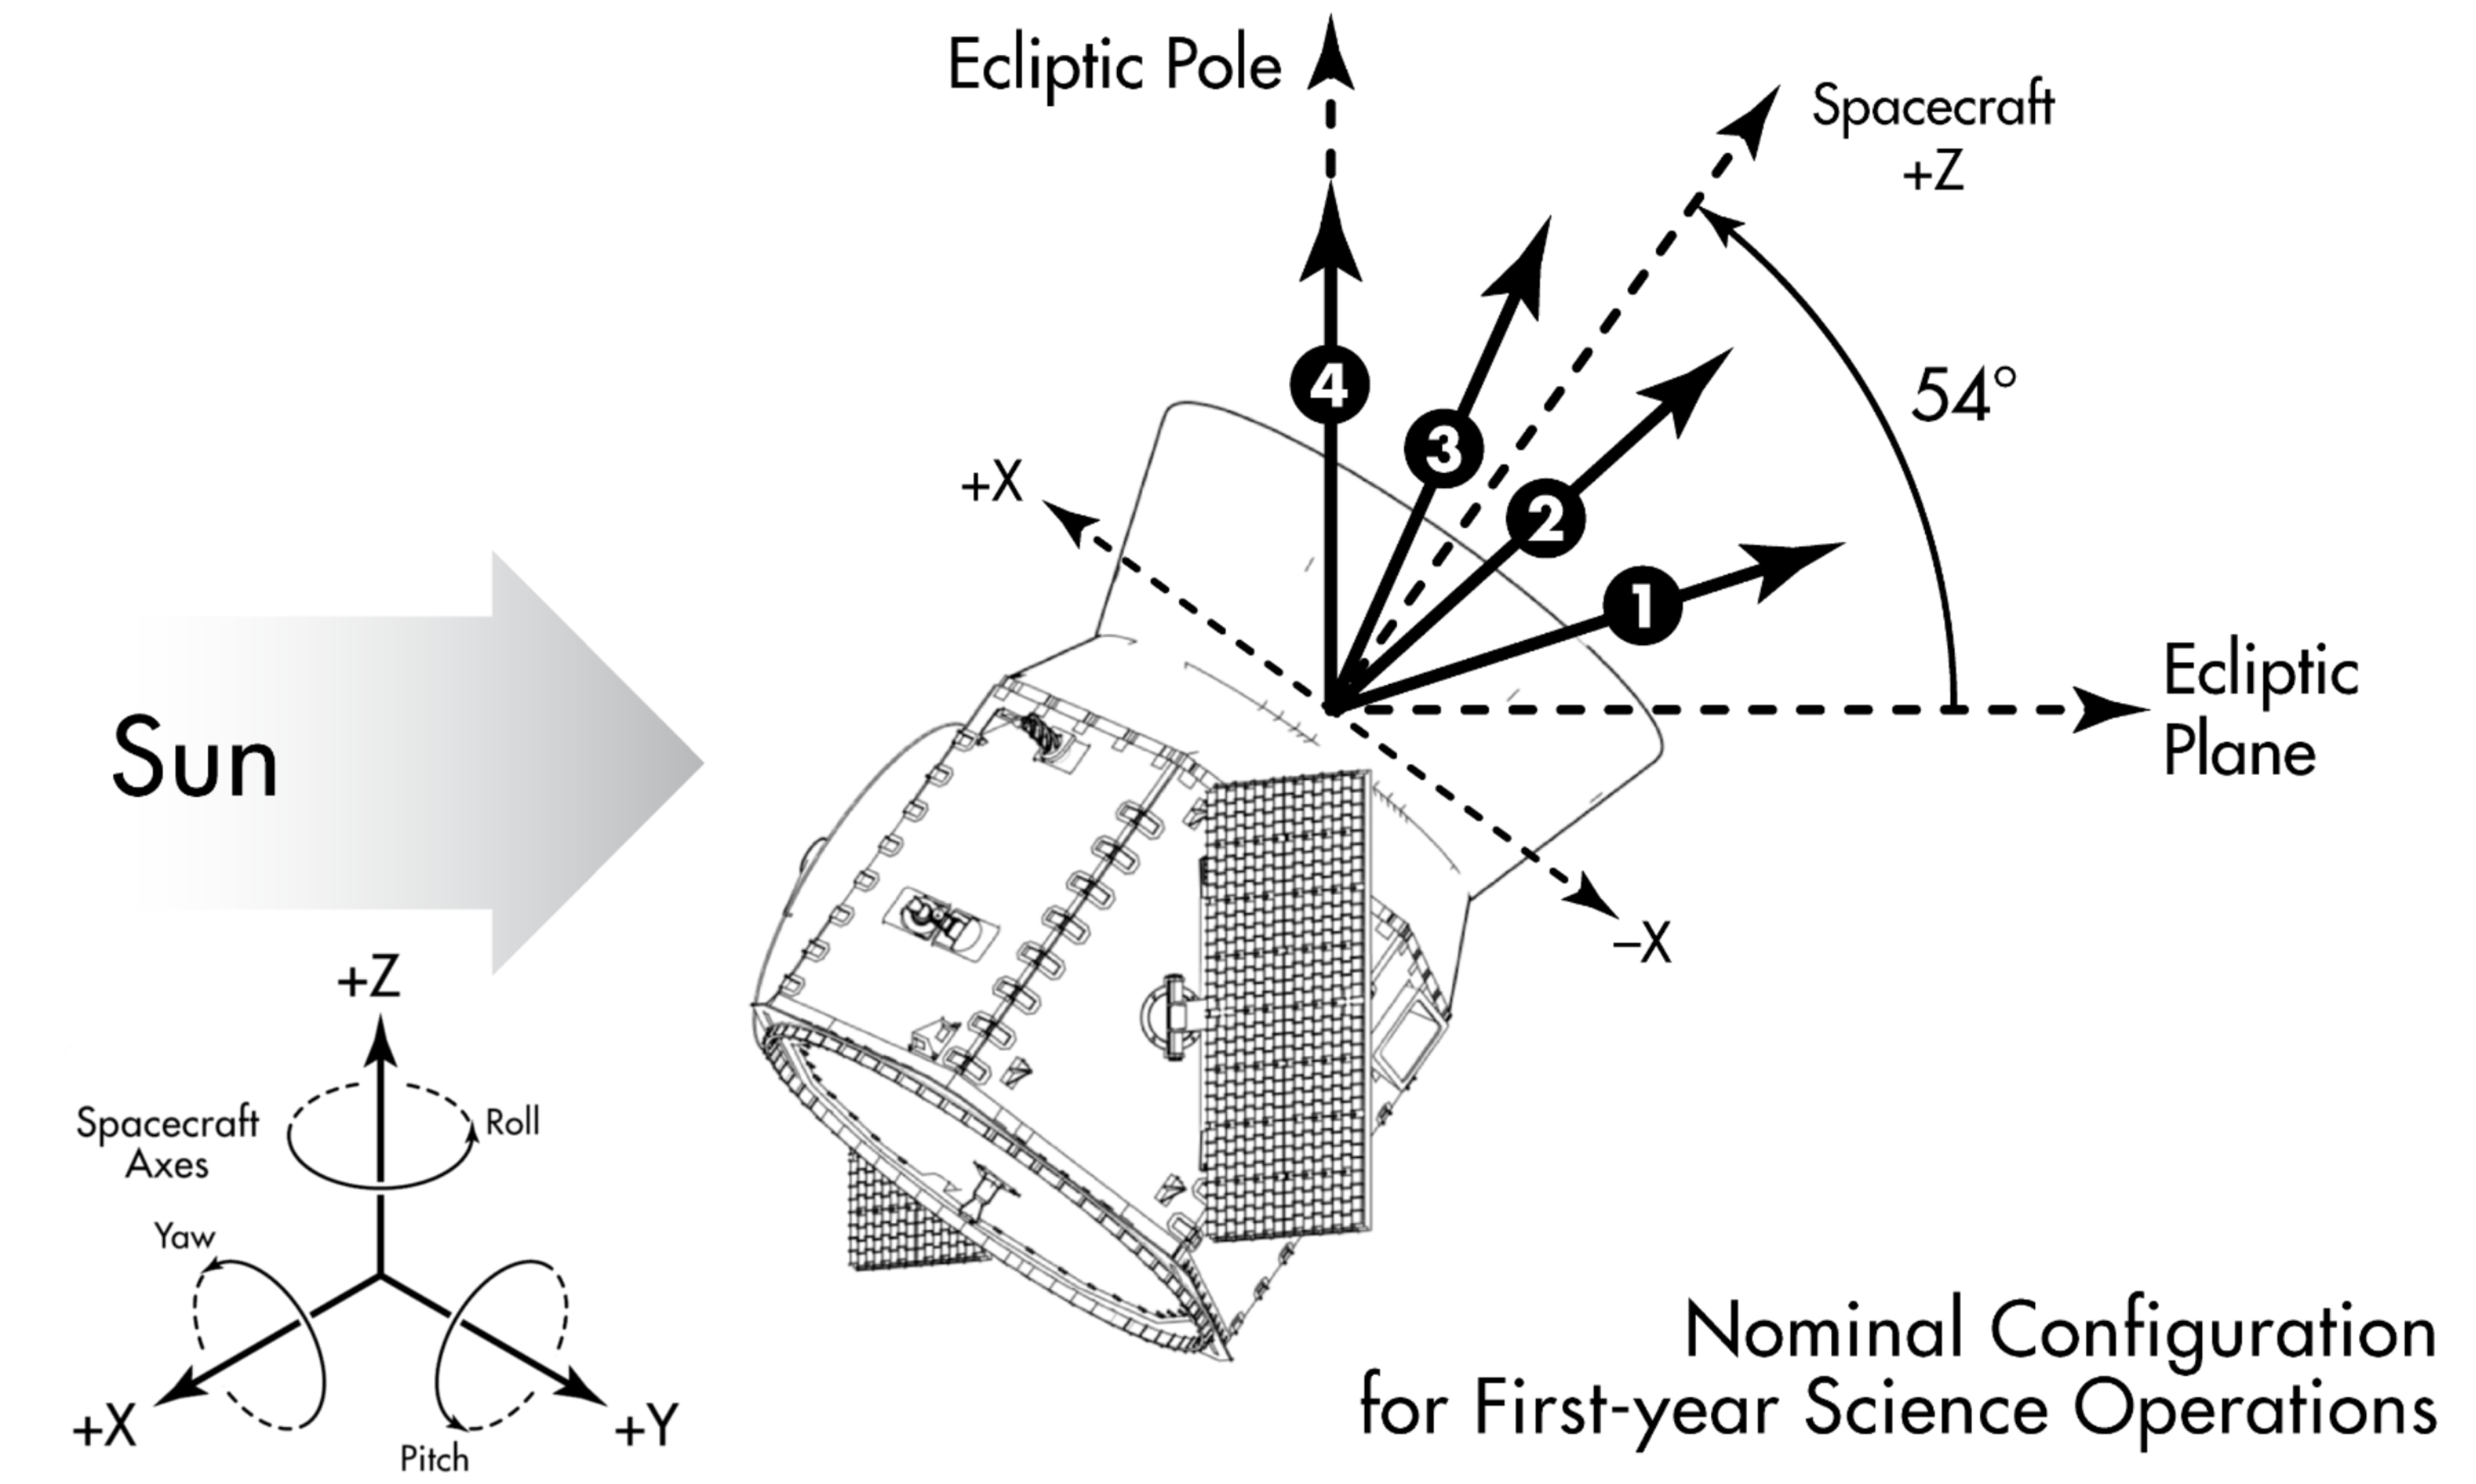
\includegraphics[width=0.9\textwidth]{../figures/spacecraft_angles.pdf}
		\caption{The spacecraft must point so that incident sunlight is collected 
			by the solar panels, and not the cameras. TESS's solar panels pitch 
			about the $+Y$ axis. (Adapted from Orbital ATK design document) }
		\label{fig:spacecraft_angles}
	\end{figure}

	\begin{figure}[!b]
		\centering
		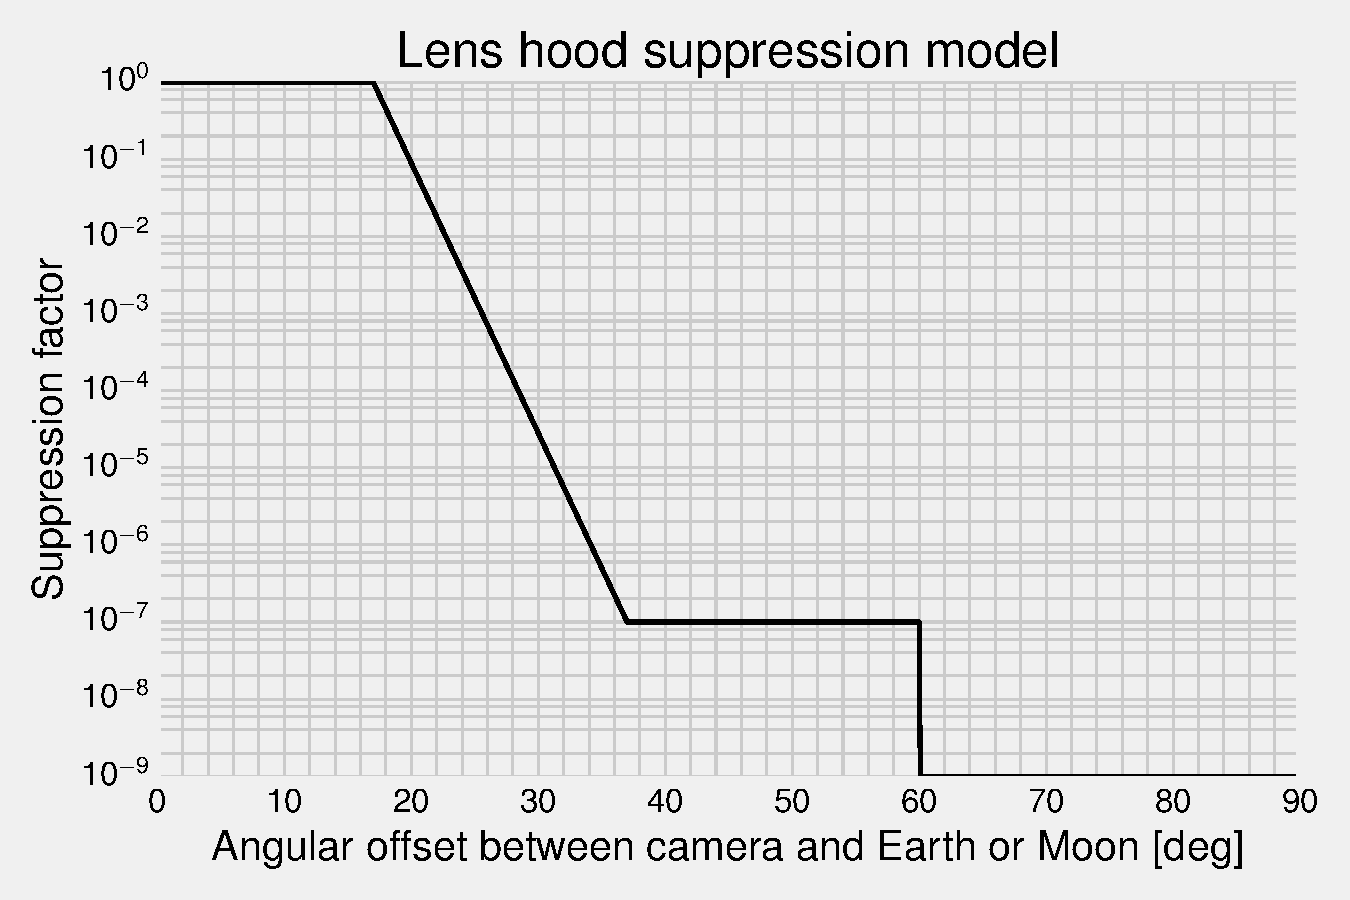
\includegraphics[width=0.9\textwidth]{../figures/lens_hood_suppression.pdf}
		\caption{TESS's lens hood suppression. }
		\label{fig:lens_hood_suppression}
	\end{figure}

\end{document}